% Capitolo 4: Rappresentazione della Conoscenza

\chapter{Rappresentazione della Conoscenza}
\label{cap:rappresentazione_conoscenza}

\section{Introduzione}

La rappresentazione della conoscenza è il problema centrale dell'intelligenza artificiale simbolica: come codificare fatti, regole, relazioni e concetti in una forma che un computer possa manipolare per ragionare e prendere decisioni.

\subsection{Requisiti Fondamentali}

Un buon schema di rappresentazione deve essere:

\begin{infobox}[Proprietà Desiderabili]
\begin{itemize}
\item \textbf{Espressivo}: capace di rappresentare la conoscenza del dominio
\item \textbf{Sintetico}: conciso e leggibile
\item \textbf{Efficiente}: manipolabile computazionalmente
\item \textbf{Modulare}: organizzabile e componibile
\item \textbf{Incrementale}: estendibile senza ristrutturazioni
\item \textbf{Dichiarativo}: separazione tra cosa e come
\end{itemize}
\end{infobox}

\section{Paradigmi di Rappresentazione}

\subsection{Logica}

La rappresentazione più formale, basata su formule logiche.

\textbf{Vantaggi}:
\begin{itemize}
\item Semantica matematica precisa
\item Correttezza e completezza dimostrabili
\item Meccanismi di inferenza ben definiti
\end{itemize}

\textbf{Svantaggi}:
\begin{itemize}
\item Difficoltà di esprimere incertezza
\item Complessità computazionale elevata
\item Monotonia (difficoltà con eccezioni)
\end{itemize}

\subsection{Reti Semantiche}

Grafi diretti dove:
\begin{itemize}
\item \textbf{Nodi} rappresentano concetti
\item \textbf{Archi} rappresentano relazioni
\end{itemize}

\begin{figure}[h]
\centering
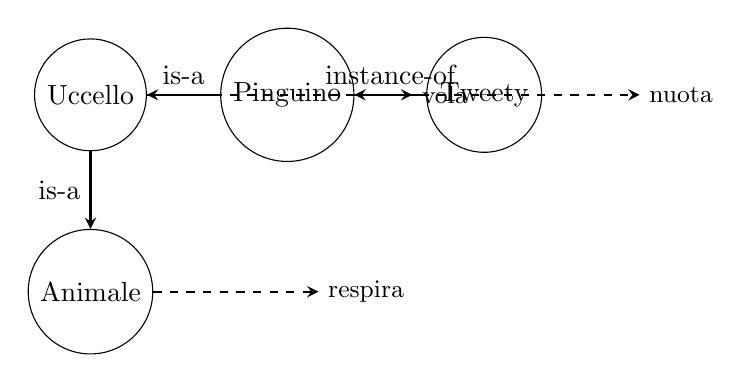
\begin{tikzpicture}[
  node distance=2.5cm,
  concept/.style={circle, draw, minimum size=1cm},
  relation/.style={->, >=stealth, thick}
]
  \node[concept] (uccello) {Uccello};
  \node[concept, right of=uccello] (pinguino) {Pinguino};
  \node[concept, below of=uccello] (animale) {Animale};
  \node[concept, right of=pinguino] (tweety) {Tweety};
  
  \draw[relation] (uccello) -- node[left] {is-a} (animale);
  \draw[relation] (pinguino) -- node[above] {is-a} (uccello);
  \draw[relation] (tweety) -- node[above] {instance-of} (pinguino);
  
  \node[right of=animale, xshift=1cm] (prop1) {\small respira};
  \node[right of=uccello, xshift=2cm] (prop2) {\small vola};
  \node[right of=pinguino, xshift=2.5cm] (prop3) {\small nuota};
  
  \draw[relation, dashed] (animale) -- (prop1);
  \draw[relation, dashed] (uccello) -- (prop2);
  \draw[relation, dashed] (pinguino) -- (prop3);
\end{tikzpicture}
\caption{Rete semantica gerarchica}
\label{fig:rete_semantica}
\end{figure}

\textbf{Ereditarietà}: Le proprietà si propagano lungo gli archi \textit{is-a}.

\subsection{Frame}

Strutture dati che raggruppano conoscenza su un concetto.

\begin{definizione}[Frame]
Un frame è una collezione di \textit{slot} (attributi) con valori, restrizioni e procedure associate.
\end{definizione}

\textbf{Esempio}:
\begin{verbatim}
Frame: Automobile
  Slots:
    - modello: [tipo: STRING]
    - anno: [tipo: INTEGER, range: 1900-2025]
    - proprietario: [tipo: Persona]
    - cilindrata: [tipo: FLOAT, default: 1600]
  Methods:
    - calcola_bollo()
    - verifica_revisione()
\end{verbatim}

\subsection{Regole di Produzione}

Il paradigma adottato da CLIPS e SLIPS.

\begin{definizione}[Regola di Produzione]
Una regola di produzione ha la forma:
\begin{equation}
\text{IF condizione THEN azione}
\end{equation}
dove:
\begin{itemize}
\item \textbf{condizione} (LHS) è un pattern sui fatti
\item \textbf{azione} (RHS) modifica la working memory
\end{itemize}
\end{definizione}

\textbf{Caratteristiche}:
\begin{itemize}
\item Modularità: ogni regola è indipendente
\item Dichiaratività: esprime "cosa" non "come"
\item Forward chaining naturale
\item Pattern matching efficiente (RETE)
\end{itemize}

\section{Rappresentazione in CLIPS}

\subsection{Fatti}

\subsubsection{Fatti Ordinati}

Sequenze di campi senza struttura esplicita:

\begin{lstlisting}[language=CLIPS]
(temperatura 25)
(colore rosso verde blu)
(coordina 10.5 20.3)
\end{lstlisting}

\textbf{Pro}: Semplici e compatti \\
\textbf{Contro}: Manca semantica esplicita dei campi

\subsubsection{Fatti Non Ordinati (Deftemplate)}

Strutture con slot nominati:

\begin{lstlisting}[language=CLIPS]
(deftemplate persona
  (slot nome (type STRING))
  (slot eta (type INTEGER) (range 0 150))
  (slot professione (default "disoccupato"))
  (multislot hobby))

(persona 
  (nome "Mario Rossi") 
  (eta 35) 
  (professione "ingegnere")
  (hobby tennis lettura programmazione))
\end{lstlisting}

\textbf{Vantaggi}:
\begin{itemize}
\item Leggibilità e manutenibilità
\item Type checking
\item Valori di default
\item Validazione (range, allowed-values)
\end{itemize}

\subsection{Regole}

\begin{lstlisting}[language=CLIPS]
(defrule diagnosi-influenza
  "Diagnostica influenza in base ai sintomi"
  (declare (salience 100))
  
  ;; Pattern matching (LHS)
  (paziente (id ?id) (nome ?nome))
  (sintomo (paziente-id ?id) (tipo febbre) (valore ?temp&:(> ?temp 38)))
  (sintomo (paziente-id ?id) (tipo tosse))
  (not (diagnosi (paziente-id ?id)))
  
  =>
  
  ;; Azioni (RHS)
  (printout t "Paziente " ?nome " probabile influenza" crlf)
  (assert (diagnosi 
            (paziente-id ?id) 
            (malattia influenza)
            (confidenza 0.8))))
\end{lstlisting}

\textbf{Elementi LHS}:
\begin{itemize}
\item Pattern positivi: \texttt{(paziente ...)}
\item Negazione: \texttt{(not ...)}
\item Congiunzione: \texttt{(and ...)}
\item Disgiunzione: \texttt{(or ...)}
\item Esistenziale: \texttt{(exists ...)}
\item Test: \texttt{(test (> ?x 10))}
\end{itemize}

\subsection{Moduli}

Organizzazione della base di conoscenza in namespace separati:

\begin{lstlisting}[language=CLIPS]
(defmodule ACQUISIZIONE
  "Raccolta dati dal paziente"
  (export deftemplate sintomo paziente))

(defmodule DIAGNOSI
  "Inferenza diagnostica"
  (import ACQUISIZIONE deftemplate sintomo paziente)
  (export deftemplate diagnosi))

(defmodule TERAPIA
  "Prescrizione cura"
  (import DIAGNOSI deftemplate diagnosi))
\end{lstlisting}

\textbf{Benefici}:
\begin{itemize}
\item Incapsulamento
\item Controllo delle dipendenze
\item Scalabilità a grandi sistemi
\item Focus selettivo (focus stack)
\end{itemize}

\section{Pattern e Variabili}

\subsection{Variabili}

\textbf{Variabili singole}:
\begin{lstlisting}[language=CLIPS]
?x        ; Qualsiasi singolo valore
?nome     ; Variabile nominata
?         ; Variabile anonima (wildcard)
\end{lstlisting}

\textbf{Variabili multifield}:
\begin{lstlisting}[language=CLIPS]
$?resto   ; Zero o piu valori
$?        ; Multifield anonimo
\end{lstlisting}

\subsection{Constraint sui Pattern}

\textbf{Predicati}:
\begin{lstlisting}[language=CLIPS]
?x&:(> ?x 10)           ; Valore > 10
?nome&:(eq ?nome "Mario")  ; Valore specifico
?y&:(numberp ?y)        ; Test di tipo
\end{lstlisting}

\textbf{Connettivi}:
\begin{lstlisting}[language=CLIPS]
?x&~nil                 ; Diverso da nil
?x&blue|red|green       ; Uno dei valori
?x&~?y                  ; Diverso da ?y
\end{lstlisting}

\subsection{Binding e Unificazione}

Quando un pattern matcha un fatto:

\begin{enumerate}
\item \textbf{Unificazione}: trovare sostituzioni $\theta$ per variabili
\item \textbf{Binding}: assegnare valori alle variabili
\item \textbf{Consistenza}: verificare constraint
\end{enumerate}

\textbf{Esempio}:
\begin{lstlisting}[language=CLIPS]
;; Pattern
(persona (nome ?n) (eta ?e&:(> ?e 18)) (citta "Roma"))

;; Fatto
(persona (nome "Giulia") (eta 25) (citta "Roma"))

;; Binding risultante
{?n -> "Giulia", ?e -> 25}
\end{lstlisting}

\section{Semantica Dichiarativa vs Procedurale}

\subsection{Interpretazione Dichiarativa}

Le regole esprimono \textit{conoscenza} generale del dominio:

\begin{lstlisting}[language=CLIPS]
(defrule sconti-anziani
  (persona (eta ?e&:(>= ?e 65)))
  =>
  (assert (sconto 20)))
\end{lstlisting}

Significato: "Le persone con 65+ anni hanno diritto a uno sconto del 20\%"

\subsection{Interpretazione Procedurale}

Le stesse regole definiscono un \textit{algoritmo} implicito:

\begin{enumerate}
\item Match delle regole applicabili
\item Conflict resolution (strategia)
\item Esecuzione (firing)
\item Ripeti fino a quiescenza
\end{enumerate}

\subsection{Dualità}

Questa dualità è una forza dei sistemi esperti basati su regole:
\begin{itemize}
\item \textbf{Esperti del dominio} vedono conoscenza dichiarativa
\item \textbf{Il sistema} esegue proceduralmente
\item \textbf{Modifiche} facili: aggiungere/rimuovere regole
\end{itemize}

\section{Chiusura del Mondo e Negazione}

\subsection{Open World Assumption (OWA)}

Nella logica classica, l'assenza di informazione significa \textit{sconosciuto}:
\begin{equation}
\Gamma \not\vdash \varphi \not\Rightarrow \Gamma \vdash \neg \varphi
\end{equation}

\subsection{Closed World Assumption (CWA)}

In CLIPS (e database), l'assenza significa \textit{falso}:
\begin{equation}
\Gamma \not\vdash \varphi \Rightarrow \Gamma \vdash \neg \varphi
\end{equation}

\subsection{Negazione in CLIPS}

\begin{lstlisting}[language=CLIPS]
(defrule nuovi-clienti
  (cliente (id ?id))
  (not (ordine (cliente-id ?id)))  ; CWA: nessun ordine = falso
  =>
  (printout t "Nuovo cliente: " ?id crlf))
\end{lstlisting}

\textbf{Attenzione}: La negazione è \textit{non monotona}:
\begin{itemize}
\item Inizialmente: nessun ordine $\Rightarrow$ regola applicabile
\item Dopo assert di ordine: regola non più applicabile
\item Truth Maintenance necessario in alcuni casi
\end{itemize}

\section{Gerarche e Ereditarietà}

\subsection{Ereditarietà via Regole}

CLIPS non ha ereditarietà built-in, ma si può simulare:

\begin{lstlisting}[language=CLIPS]
;; Gerarchia esplicita
(deffacts tassonomia
  (is-a cane mammifero)
  (is-a gatto mammifero)
  (is-a mammifero animale)
  (is-a animale essere-vivente))

;; Propagazione proprieta
(defrule eredita-proprieta
  (is-a ?figlio ?genitore)
  (proprieta (classe ?genitore) (attributo ?attr) (valore ?val))
  (not (proprieta (classe ?figlio) (attributo ?attr)))
  =>
  (assert (proprieta (classe ?figlio) (attributo ?attr) (valore ?val))))
\end{lstlisting}

\subsection{Overriding ed Eccezioni}

Gestione delle eccezioni tramite salience:

\begin{lstlisting}[language=CLIPS]
(defrule uccelli-volano
  (declare (salience 10))
  (animale (tipo uccello) (nome ?n))
  =>
  (assert (puo-volare ?n)))

(defrule pinguini-non-volano
  (declare (salience 20))  ; Priorita maggiore!
  (animale (tipo pinguino) (nome ?n))
  =>
  (assert (non-puo-volare ?n)))
\end{lstlisting}

\section{Conoscenza Temporale}

\subsection{Rappresentazione dello Stato}

\textbf{Approccio 1: Stato Implicito} (Working Memory = stato corrente)

\begin{lstlisting}[language=CLIPS]
(temperatura 25)
(ora 14:30)
\end{lstlisting}

\textbf{Approccio 2: Stato Esplicito con Timestamp}

\begin{lstlisting}[language=CLIPS]
(deftemplate misura
  (slot parametro)
  (slot valore)
  (slot timestamp))

(misura (parametro temperatura) (valore 25) (timestamp 1445))
(misura (parametro temperatura) (valore 26) (timestamp 1450))
\end{lstlisting}

\subsection{Eventi e Transizioni}

\begin{lstlisting}[language=CLIPS]
(deftemplate evento
  (slot tipo)
  (slot tempo)
  (multislot dati))

(defrule rileva-anomalia
  (evento (tipo misura) (tempo ?t1) (dati temperatura ?temp1))
  (evento (tipo misura) (tempo ?t2&:(> ?t2 ?t1)) (dati temperatura ?temp2))
  (test (> (abs (- ?temp2 ?temp1)) 10))
  =>
  (assert (allarme (tipo variazione-rapida) (tempo ?t2))))
\end{lstlisting}

\section{Conoscenza Incerta}

\subsection{Fattori di Certezza (Certainty Factors)}

Approccio MYCIN:

\begin{lstlisting}[language=CLIPS]
(deftemplate ipotesi
  (slot diagnosi)
  (slot cf (type FLOAT) (range -1.0 1.0)))

(defrule combina-evidenze
  (sintomo (tipo ?s1) (cf ?cf1))
  (regola (se ?s1) (allora ?diagnosi) (cf-regola ?cfr))
  =>
  (bind ?cf-combinato (* ?cf1 ?cfr))
  (assert (ipotesi (diagnosi ?diagnosi) (cf ?cf-combinato))))
\end{lstlisting}

\subsection{Logica Fuzzy}

CLIPS supporta FuzzyCLIPS per logica sfumata:

\begin{verbatim}
(deftemplate temperatura
  0 100 gradi
  ((fredda (z 10 20))
   (mite (pi 15 25))
   (calda (s 20 30))))
\end{verbatim}

\section{Meta-Conoscenza}

\subsection{Conoscenza sulla Conoscenza}

\begin{lstlisting}[language=CLIPS]
(deftemplate regola-meta
  (slot id-regola)
  (slot applicabilita (allowed-values alta media bassa))
  (slot confidenza (type FLOAT))
  (slot fonte))

;; Decidere quando applicare una regola
(defrule usa-regola-affidabile
  (regola-meta (id-regola ?r) (confidenza ?c&:(> ?c 0.8)))
  (agenda ?r ...)
  =>
  (fire ?r))
\end{lstlisting}

\subsection{Strategia Dinamica}

\begin{lstlisting}[language=CLIPS]
(defrule cambia-strategia
  (fase iniziale)
  (num-fatti ?n&:(> ?n 1000))
  =>
  (set-strategy complexity)  ; Passa a strategia per complessita
  (retract-string "(fase iniziale)")
  (assert (fase ottimizzazione)))
\end{lstlisting}

\section{Design Pattern per la Conoscenza}

\subsection{Pattern: State Machine}

\begin{lstlisting}[language=CLIPS]
(deftemplate stato
  (slot nome)
  (slot attivo (default no)))

(defrule transizione
  ?s1 <- (stato (nome ?da) (attivo yes))
  (evento (trigger ?trigger))
  (regola-transizione (da ?da) (evento ?trigger) (a ?a))
  =>
  (modify ?s1 (attivo no))
  (assert (stato (nome ?a) (attivo yes))))
\end{lstlisting}

\subsection{Pattern: Blackboard}

Spazio condiviso per cooperazione tra moduli:

\begin{lstlisting}[language=CLIPS]
(deftemplate ipotesi-blackboard
  (slot livello (allowed-values basso medio alto))
  (slot contenuto)
  (slot fonte))

;; Modulo basso livello
(defrule rileva-feature
  (segnale (dati ?d))
  =>
  (assert (ipotesi-blackboard (livello basso) (contenuto ?d))))

;; Modulo alto livello
(defrule integra-ipotesi
  (ipotesi-blackboard (livello basso) (contenuto ?c1))
  (ipotesi-blackboard (livello basso) (contenuto ?c2))
  =>
  (assert (ipotesi-blackboard (livello alto) (contenuto ...))))
\end{lstlisting}

\subsection{Pattern: Case-Based Reasoning}

\begin{lstlisting}[language=CLIPS]
(deftemplate caso
  (slot problema)
  (slot soluzione)
  (slot similarita))

(defrule recupera-caso-simile
  (problema-corrente ?p)
  (caso (problema ?pc) (soluzione ?s))
  (test (> (calcola-similarita ?p ?pc) 0.8))
  =>
  (assert (candidato-soluzione ?s)))
\end{lstlisting}

\section{Limiti e Trade-off}

\subsection{Espressività vs Efficienza}

\begin{table}[h]
\centering
\begin{tabular}{@{}lcc@{}}
\toprule
\textbf{Formalismo} & \textbf{Espressività} & \textbf{Complessità} \\
\midrule
Logica proposizionale & Bassa & P (SAT: NP-completo) \\
Clausole di Horn & Media & P (lineare) \\
FOL & Alta & Indecidibile \\
Regole produzione & Media-Alta & Efficiente con RETE \\
\bottomrule
\end{tabular}
\caption{Trade-off espressività-efficienza}
\end{table}

\subsection{Limitazioni di CLIPS}

\begin{itemize}
\item No quantificazione universale esplicita in LHS
\item No funzioni higher-order
\item No backtracking (ricerca non esaustiva)
\item No constraint propagation automatica
\item Gestione limitata dell'incertezza
\end{itemize}

\subsection{Quando Usare Altri Formalismi}

\begin{itemize}
\item \textbf{Description Logic} (OWL): ontologie, ragionamento subsumption
\item \textbf{Answer Set Programming}: ottimizzazione combinatoria
\item \textbf{Probabilistic Graphical Models}: incertezza, apprendimento
\item \textbf{Constraint Programming}: scheduling, planning
\end{itemize}

\section{Best Practices}

\subsection{Principi di Buona Modellazione}

\begin{infobox}[Linee Guida]
\begin{enumerate}
\item \textbf{Atomicità}: Un fatto = una informazione atomica
\item \textbf{Normalizzazione}: Evitare ridondanza
\item \textbf{Naming conventions}: Nomi descrittivi e consistenti
\item \textbf{Documentazione}: Commenti per regole complesse
\item \textbf{Modularità}: Usare defmodule per organizzazione
\item \textbf{Testing}: Verificare regole indipendentemente
\end{enumerate}
\end{infobox}

\subsection{Antipattern da Evitare}

\begin{warningbox}[Errori Comuni]
\begin{itemize}
\item \textbf{God rules}: Regole che fanno troppe cose
\item \textbf{Hardcoding}: Valori letterali invece di parametri
\item \textbf{Negazione imprudente}: Può causare loop
\item \textbf{Salience abuse}: Troppa dipendenza da priorità esplicite
\item \textbf{Global state nascosto}: Effetti collaterali non dichiarati
\end{itemize}
\end{warningbox}

\section{Conclusioni del Capitolo}

\subsection{Punti Chiave}

\begin{enumerate}
\item La rappresentazione della conoscenza è cruciale per sistemi efficaci
\item CLIPS offre un buon bilanciamento tra espressività ed efficienza
\item I deftemplate forniscono struttura e validazione
\item I moduli permettono scalabilità
\item Pattern matching unifica dichiaratività e computazione
\end{enumerate}

\subsection{Implicazioni per SLIPS}

SLIPS deve preservare fedelmente:
\begin{itemize}
\item Semantica dei deftemplate e dei fatti
\item Comportamento dell'unificazione e binding
\item Gestione della negazione (CWA)
\item Modularità e namespace
\item Interazione tra rappresentazione e inferenza
\end{itemize}

\subsection{Prossimi Passi}

Il Capitolo~\ref{cap:rete_introduzione} mostrerà come il pattern matching efficiente rende possibile lavorare con grandi basi di conoscenza rappresentate come regole.

\subsection{Letture Consigliate}

\begin{itemize}
\item \textit{Knowledge Representation and Reasoning} - Brachman \& Levesque (2004)
\item \textit{Principles of Knowledge Representation} - Sowa (1999)
\item \textit{Semantic Web for the Working Ontologist} - Allemang \& Hendler (2011)
\item CLIPS Reference Manual - Capitoli 2-5
\item \textit{Expert Systems: Principles and Programming} - Giarratano \& Riley (2004)
\end{itemize}
